The main purpose behind this project was to reproduce the results obtained by Zanghellini et al. for a 2-electron interacting system inserted in a harmonic oscillator potential illuminated by a laser source. First we will present the results obtained for the time-independent treatment, switching then to the time-dependent case at a later stage. For the whole development of the code, the radial part of the single particle wavefunctions was written using the first $l=10$ eigenstates $\chi_\mu$ of the harmonic oscillator hamiltonian, entering into Eq.\,\ref{eq:expansion_spf_gen} and Eq.\,\ref{eq:expansion_spf_res}. Each $\chi_\mu$ was evaluated on a mesh of 201 points covering the interval (-10, 10), as specified in the mentioned article. All the results reported below were derived by imposing the initial coefficient matrix equal to an identity matrix with proper dimensionality, namely $2l\times 2l$ and $l\times l$ respectively for the general and restricted solvers. We recall that the natural units convention has been employed, thus all the results reported below are represented in these reduced units.


\subsection{TIME-INDEPENDENT TREATMENT}
As introduced above, the comparison with the results by Zanghellini et al. regarded two main features of the system's ground state, which are the energy and the one-body density. We started by solving the Ruthaan-Hall equations with $\delta=10^{-6}$, adopting both the general and restricted Hartree-Fock solvers. The so-obtained coefficients for the ground state were exploited for the evaluation of the energy and the expected value for the position operator, defined respectively in Eq.\,\ref{eq:total_energy_coeff} and \ref{eq:x_time_dependent_coeff}. The corresponding estimations are reported in Table \ref{tab:E_x_comp_article}. The one-body density was also evaluated and a comparison with the result reported in the article can be found in Figure \ref{fig:one_body_density_comp}. The integral performed over these curves provided us with the values reported again in Table \ref{tab:E_x_comp_article} 

\begin{table}[h!]
    \centering
    \begin{tabular}{cccc}
        \toprule
         & Energy [Hartr.] & Dipole [a.u.] & Integral  \\
        \midrule
        Article & $1.1795$ & - & - \\
        General & $1.17957$ &  $3.539\times10^{-10}$ & $2.000$ \\
        Restric. & $1.17957$ & $1.660\times10^{-10}$ & $2.000$ \\
        \bottomrule
    \end{tabular}
    \caption{Expected values for energy and position operator in the ground state obtained by Zangellini et al. and through our code. Both the general and restricted implementation were exploited, with $\delta=10^{-6}$ and $\Omega=0.25$. }
    \label{tab:E_x_comp_article}
\end{table}



\begin{figure*}[h!]
    \centering
    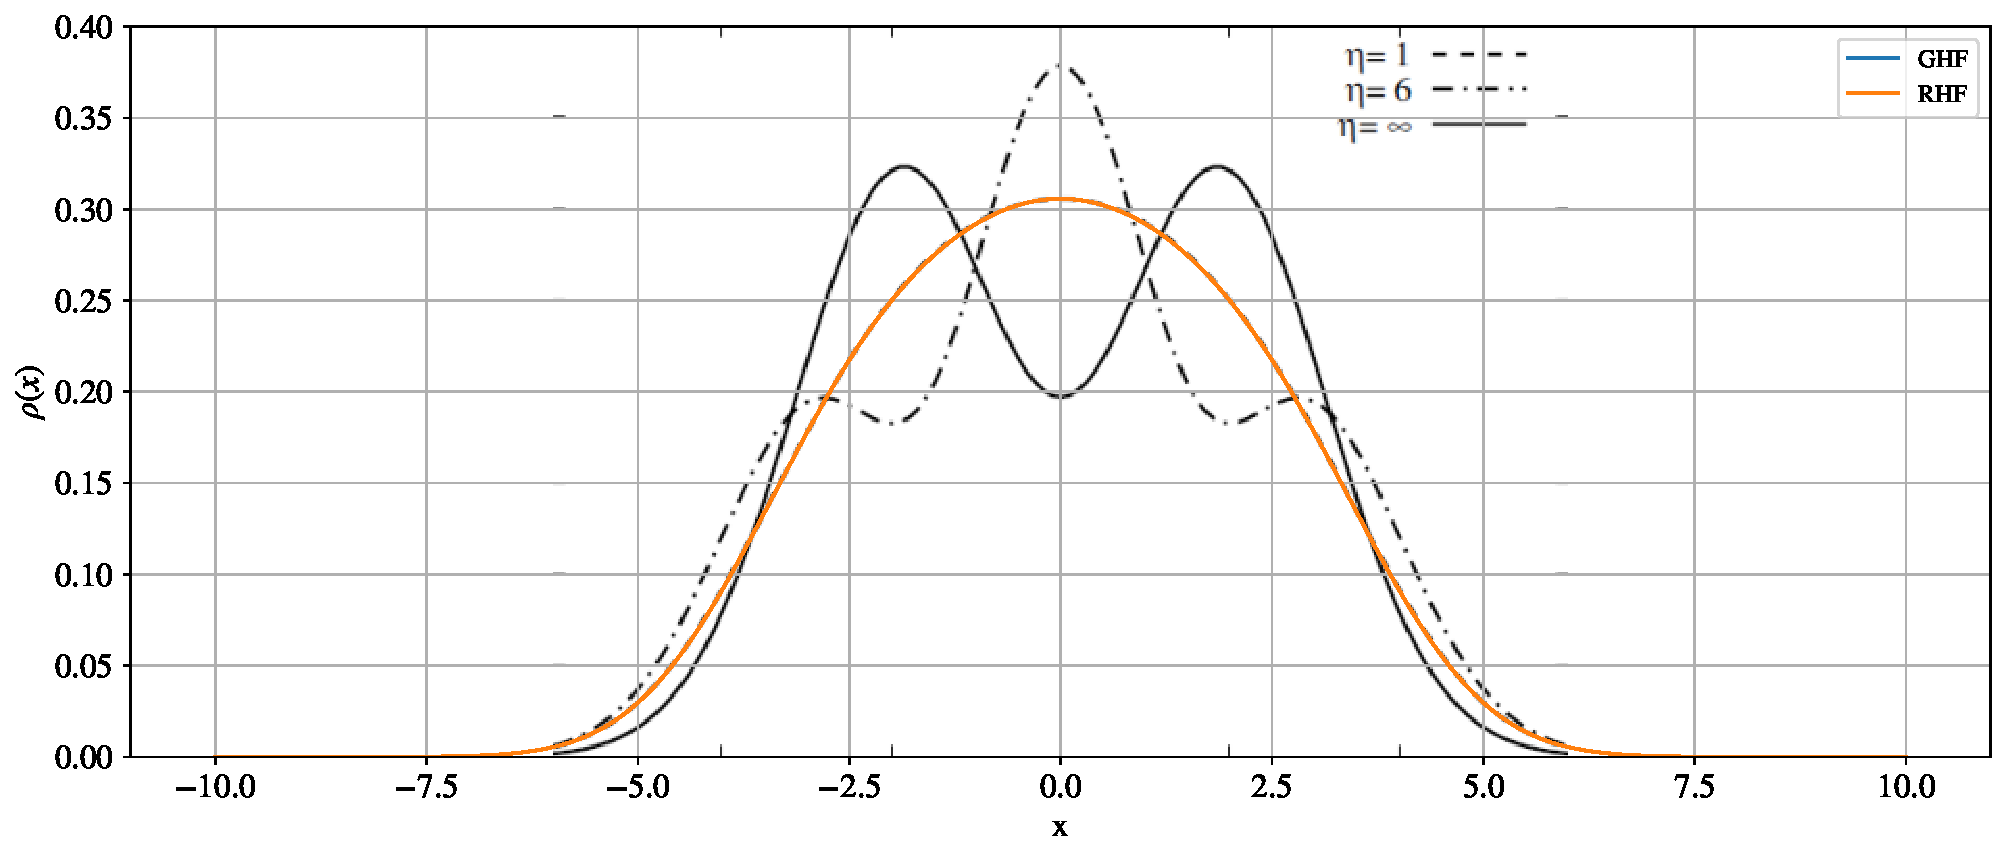
\includegraphics[scale=0.5]{images/onebody_density_comp_article.pdf}
    \caption{Comparison between our estimates for the ground state one-body density and the corresponding result in \cite{Zanghellini_2004} for a system with $\Omega=0.25$ . The obtained curves (which are perfectly overlapped) were produced exploiting the matrix coefficients provided by the convergence of the Ruthaan-Hall equations with $\delta=10^{-6}$, respectively in the general and restricted representation.}
    \label{fig:one_body_density_comp}
\end{figure*}

In order to appreciate possible differences between the general and restricted approach, we launched other simulations with the corresponding time-independent Hartree-Fock solvers, but this time stopping the algorithm after fixed number of $100$ iterations instead of looking at the tolerance $\delta$. In particular, a properly implemented function returned the total energy of the system and the parameter $\Delta$ (see Eq.\,\ref{eq:stop_condition}) evaluated at every step, providing the results shown in Figure \ref{fig:energy_at_every_step} and Figure \ref{fig:delta_at_every_step}.

\begin{figure}[t!]
    \centering
    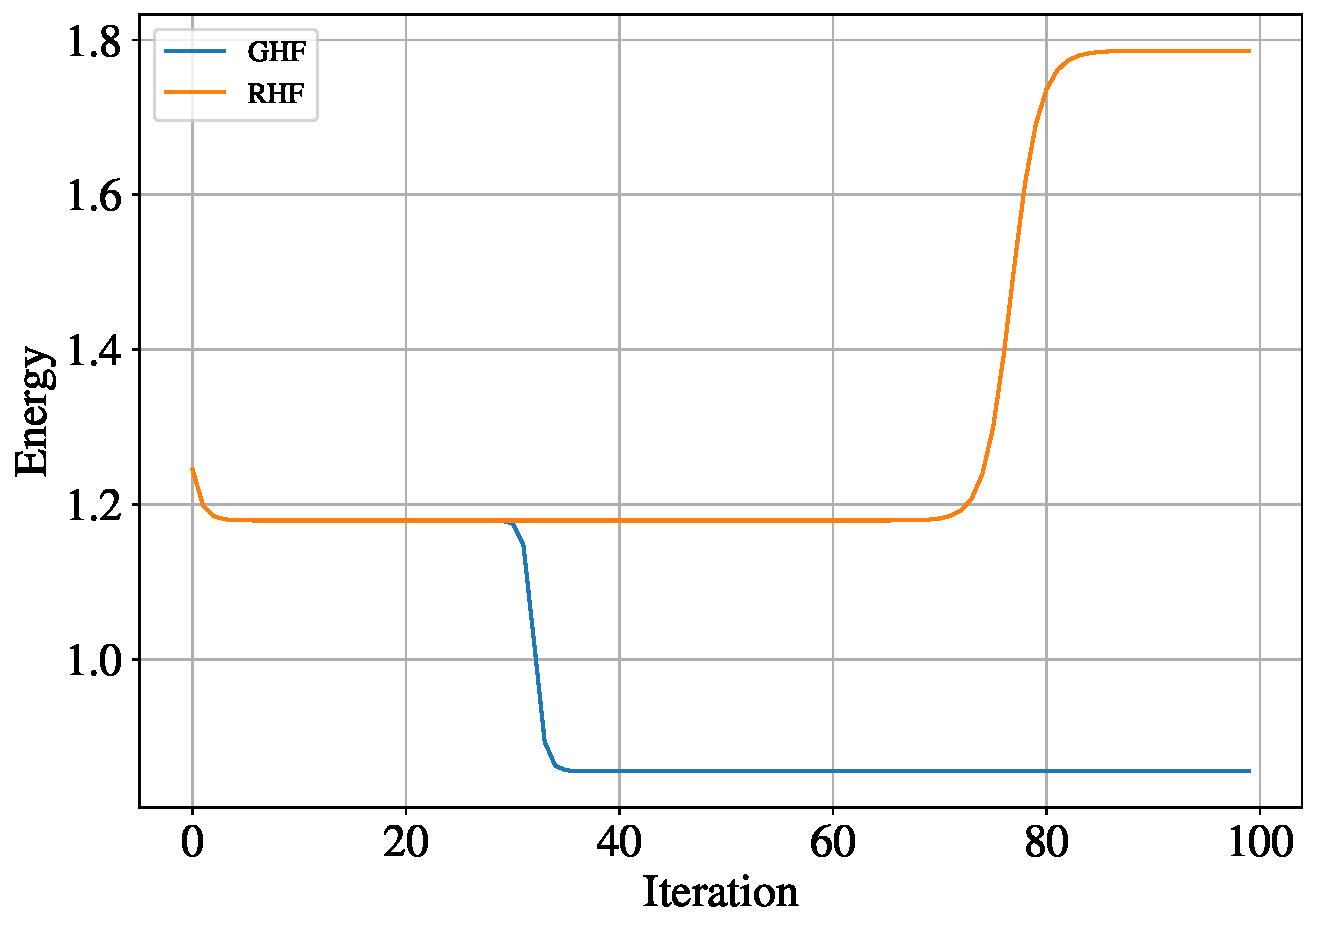
\includegraphics[scale=0.38]{images/energy_at_every_step.pdf}
    \caption{Total energy obtained for each iteration of the time-independent Hartree-Fock solver respectively in the general and restricted representation for a system with $\Omega=0.25$.}
    \label{fig:energy_at_every_step}
\end{figure}

\begin{figure}[t!]
    \centering
    \hspace{-15pt}
    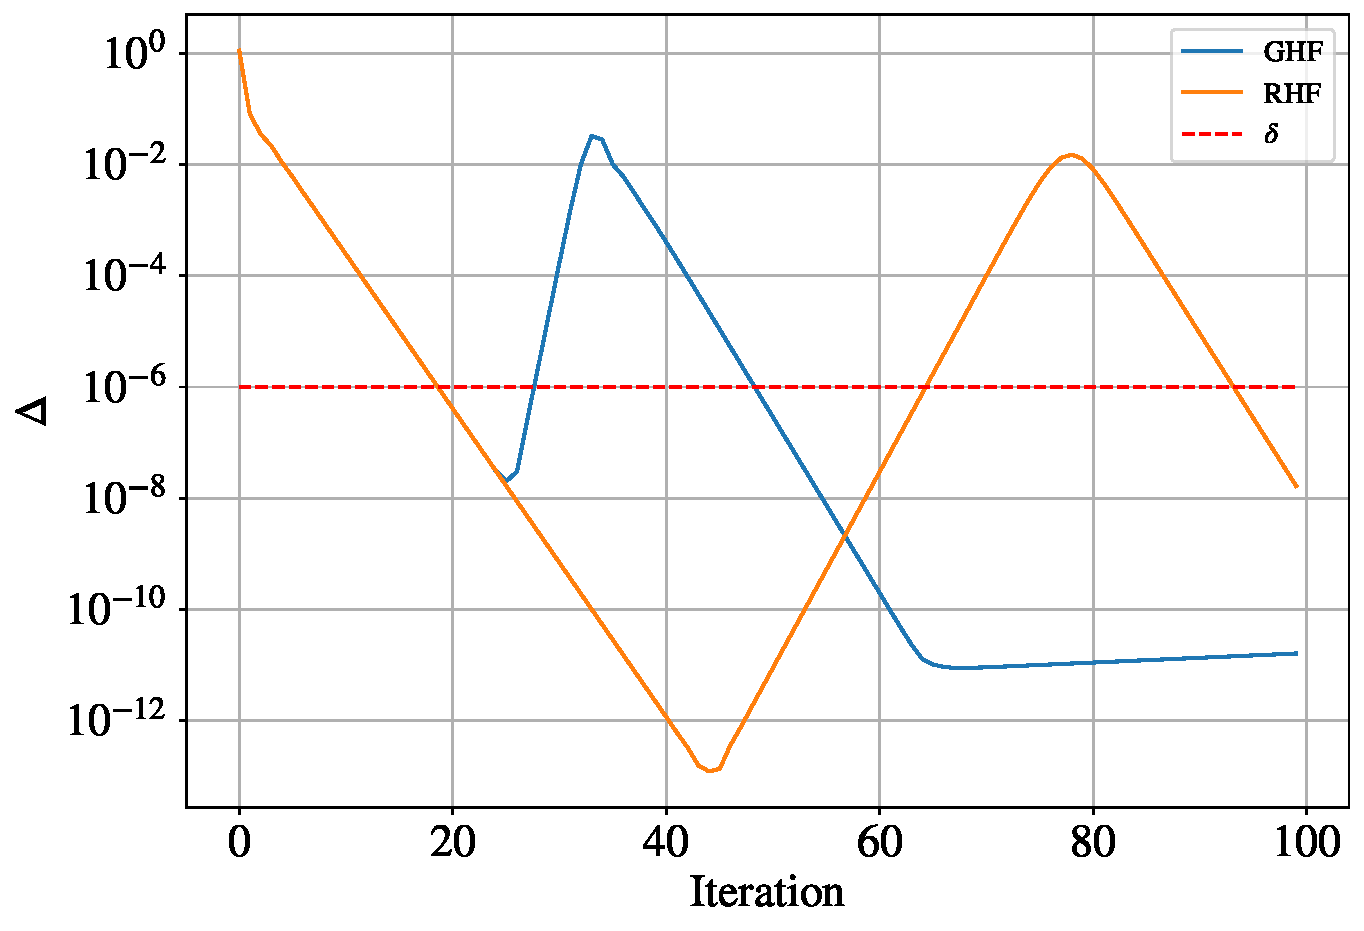
\includegraphics[scale=0.38]{images/delta_at_every_step.pdf}
    \caption{$\Delta$ parameter (see Eq.\,\ref{eq:stop_condition}) evaluated for each iteration of the time-independent Hartree-Fock solver respectively in the general and restricted representation for a system with $\Omega=0.25$. The dashed line represents the threshold value chosen for $\delta$ for the simulations carried out in the context of this project.}
    \label{fig:delta_at_every_step}
\end{figure}



\subsection{TIME-DEPENDENT TREATMENT}
Switching to the time-dependent case, now the comparison with the article by Zanghellini is focused on the overlap between the wavefunction evaluated at $t=0$ and $t\neq 0$, expressed by the parameter $\xi(t)$ defined in Eq.\,\ref{eq:overlap_coeff}. From now on, only the results provided by the general solver will be taken into consideration. In order to reproduce the plots reported in the paper, we exploited the coefficient matrix for the ground state evaluated in the time-independent framework with $\Omega=0.25$ and $\delta=10^{-6}$, using these as a seed for the integrator described in Section \ref{sec:integrator}. We employed a time step $dt=10^{-4}$, allowing for a good compromise between speed and accuracy. Also smaller values for the time step were tested, but they didn't provide any evident improvement in this sense. In addition to the overlap, also the time-evolution of the dipole operator was included in the analysis by inserting into Eq.\,\ref{eq:x_time_dependent_coeff} the coefficient matrix provided by the integrator at each time instant. The results are reported respectively in Figure \ref{fig:overlap_comp_paper} and Figure \ref{fig:dipole_comp}. The procedures described up to now were also applied to other $\omega$ values, the corresponding plots being reported in Figure \ref{fig:overlap_comp_omega} and Figure \ref{fig:dipole_comp} for a comparison with the standard case of $\omega=2$. The one-body density time evolution was also represented together with the behaviour of the one-body potential: these results for the mentioned $\omega$ configurations appear in some animated pictures that one can find \href{https://github.com/Matteo294/FYS4411/tree/main/Project2/code}{here}.  \\

\begin{figure*}[h!]
    \centering
    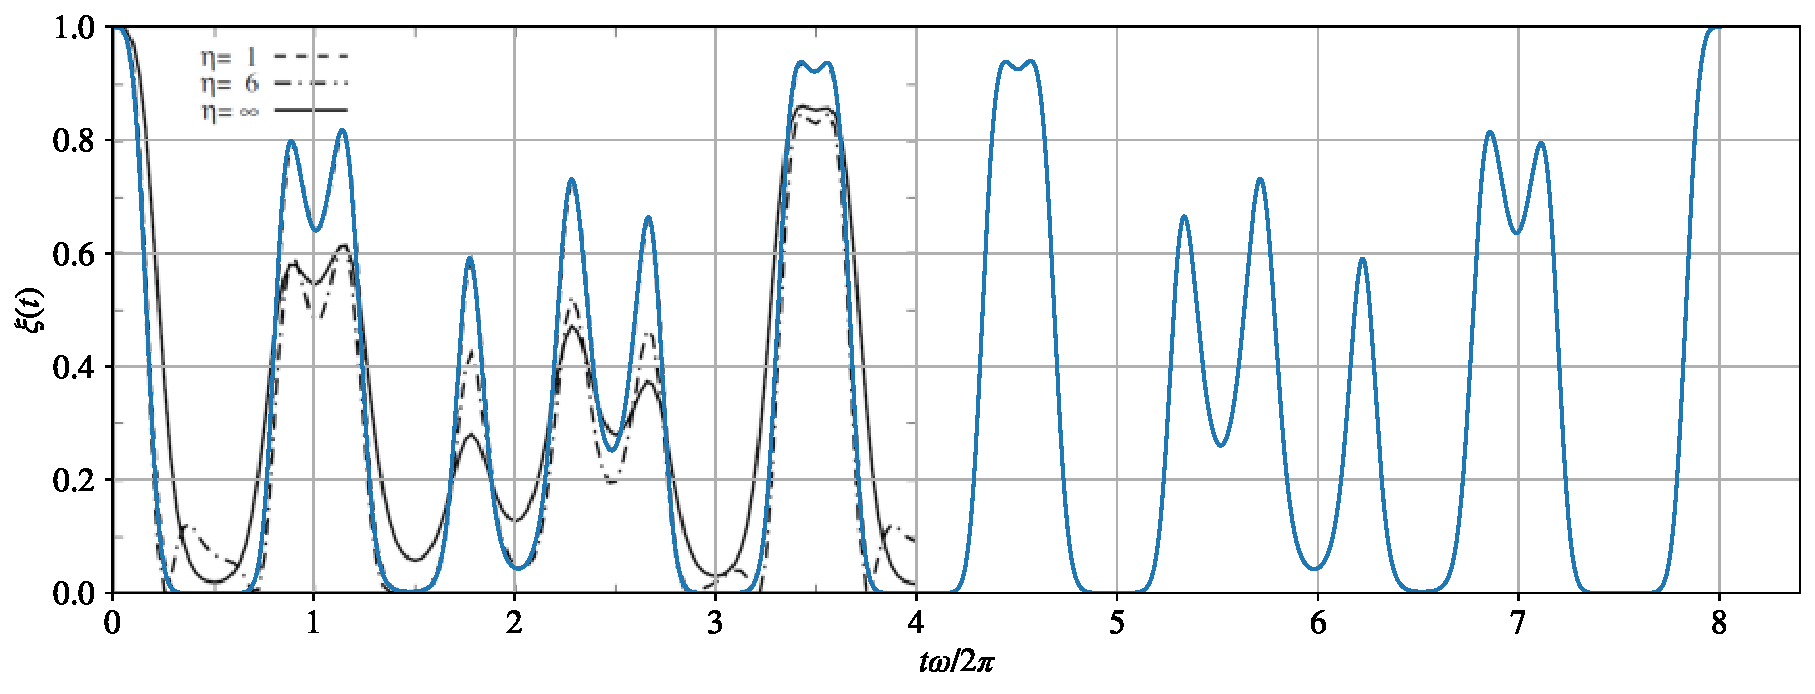
\includegraphics[scale=0.5]{images/overlap_comp_article.pdf}
    \caption{Comparison between the time-evolution of the overlap $\xi(t)$ (see Eq.\,\ref{eq:overlap_coeff}) provided by our code and the corresponding result reported in \cite{Zanghellini_2004} for a system with $\Omega=0.25$ and $\omega=2$, using a time step $\delta t=10^{-4}$. The coefficient matrix used as initial condition for the time evolution corresponds to the resulting one from the convergence of the time-independent solver with $\delta=10^{-6}$. }
    \label{fig:overlap_comp_paper}
\end{figure*}

\begin{figure*}[h!]
    \centering
    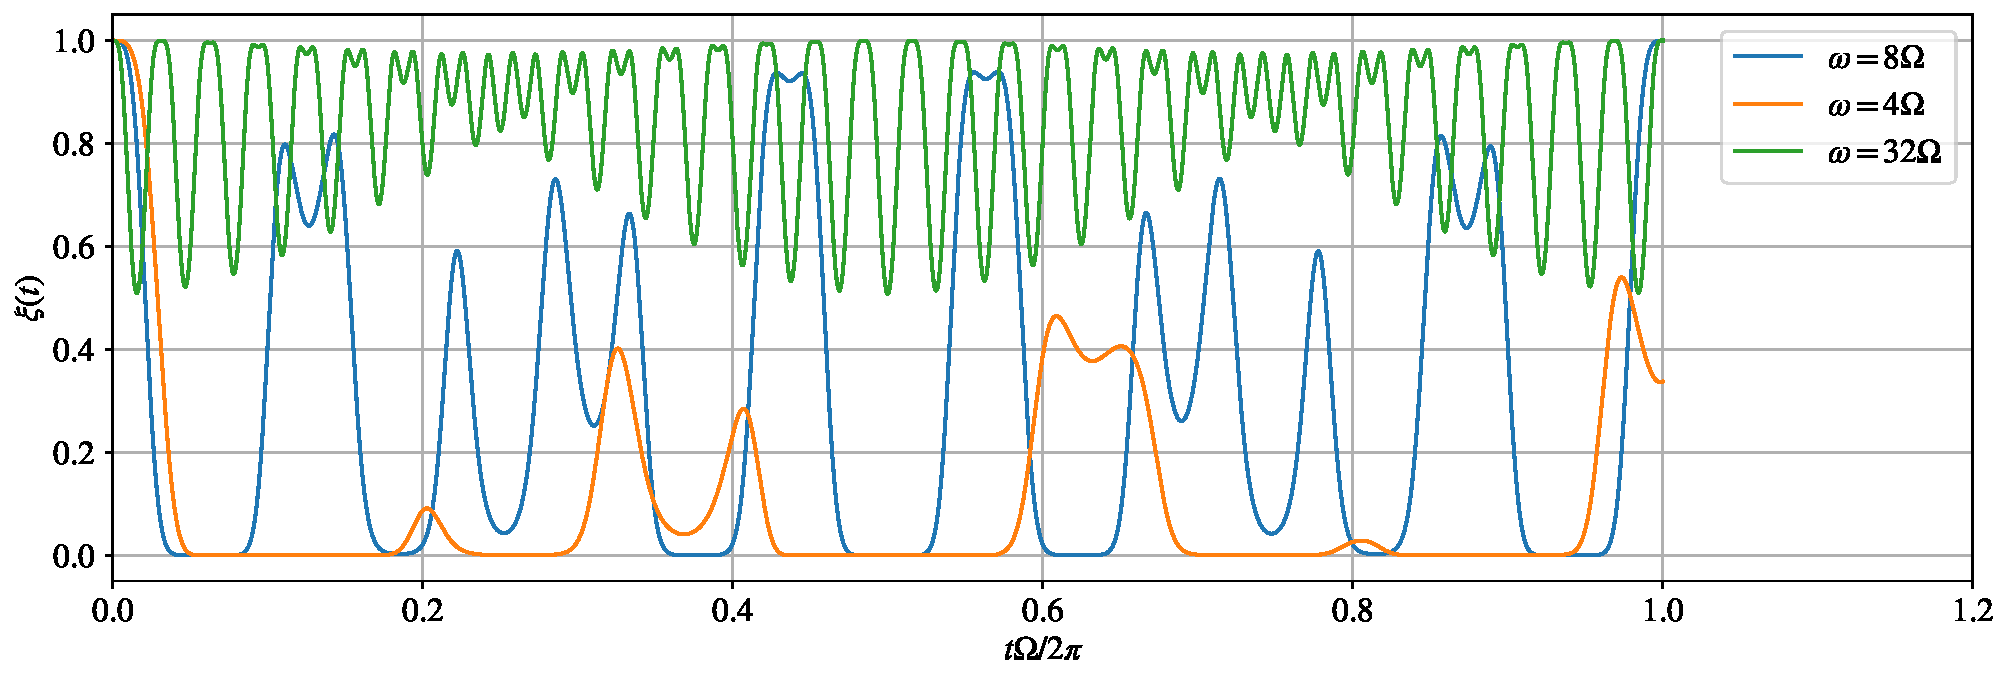
\includegraphics[scale=0.5]{images/overlaps_different_omega.pdf}
    \caption{Comparison between the time-evolution of the overlap $\xi(t)$ (see Eq.\,\ref{eq:overlap_coeff}) provided by our code for $\Omega=0.25$ and different values for $\omega$, using $\delta t = 10^{-4}$. The coefficient matrix used as initial condition for the time evolution corresponds to the resulting one from the convergence of the time-independent solver with $\delta=10^{-6}$.}
    \label{fig:overlap_comp_omega}
\end{figure*}

\begin{figure}[t!]
    \centering
    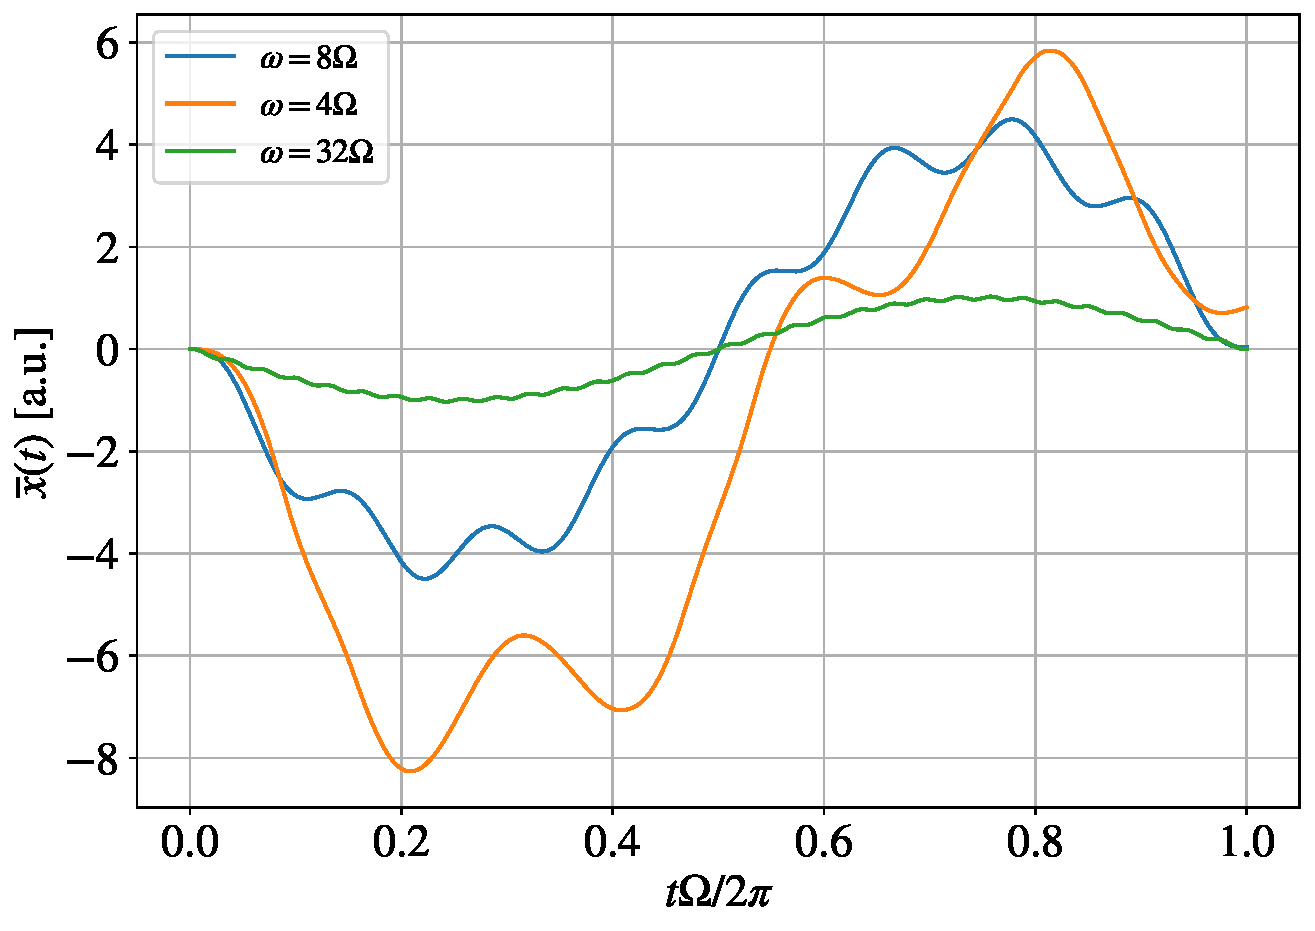
\includegraphics[scale=0.38]{images/dipoles_different_omega.pdf}
    \caption{Time evolution of the dipole operator $\overline{x}(t)$ (see Eq.\,\ref{eq:x_time_dependent_coeff}) for a system with $\Omega=0.25$ and three different $\omega$ values, using $\delta t = 10^{-4}$. The coefficient matrix used as initial condition for the time evolution corresponds to the resulting one from the convergence of the time-independent solver with $\delta=10^{-6}$.}
    \label{fig:dipole_comp}
\end{figure}


Finally, we report the results obtained in the context of the Fourier analysis described in Section \ref{sec:fourier_analysis}. For this purpose, we launched a time-evolution of the system with the laser source active for a time $T=10\pi$, then the simulation proceeded with the laser turned off until $T_f = 100\pi$. For the simulation we adopted $dt=10^{-4}$, evaluating at each instant the parameters $\xi_T(t)$ and $\overline{x}(t)$ defined in Eq.\,\ref{eq:overlap_T_coeff} and Eq.\,\ref{eq:x_time_dependent_coeff}. The points of these curves obtained for $t\in (T,T_f)$ were then processed with the FFT algorithm. In particular, the procedure described up to now was repeated for three different values of $\Omega$ and $\omega$, in order to find a possible correlation between them and the frequency components appearing in the spectrum. For each run with different $\Omega$ we exploited as seed the corresponding ground-state coefficient matrix provided by the general Hartree-Fock solver with $\delta=10^{-6}$.

For all the considered simulations, the same values for cited above for $T$ and $T_f$ were used. The curves for $\overline{x}(t)$ and $\xi_T(t)$ reported in Figure \ref{fig:laser_on_off} and Figure \ref{fig:overlap_T} are referred to $\Omega=0.25$ and $\omega=8\Omega=2$, while the spectra appearing in Figure \ref{fig:fourier_spectra_x} and Figure \ref{fig:fourier_spectra_xi} correspond to the configurations reported in the respective legends. The reliability of the implemented code was enforced by the fact that the energy of the system remained constant after the laser source was switched off.

\afterpage{
\begin{figure}[t!]
    \centering
    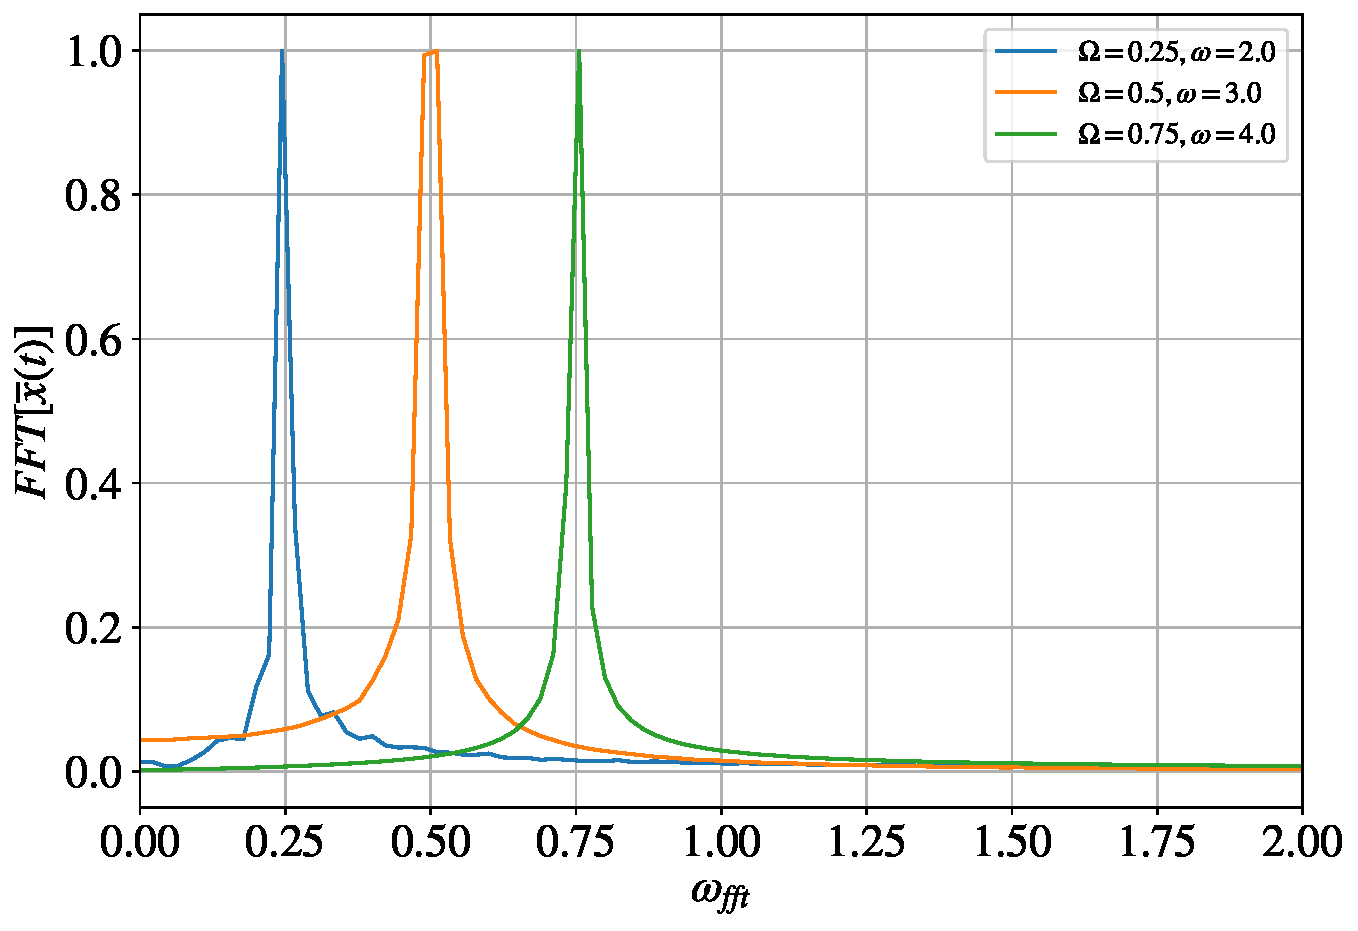
\includegraphics[scale=0.38]{images/spectra_x_diff_omegas.pdf}
    \caption{Normalized Fourier spectra of the signal $\overline{x}(t)$ with $t \in (T,T_f)$ for three different combinations of $\Omega$ and $\omega$, using $\delta t = 10^{-4}$. In each time-evolution the laser source was left active for $t \in (0, T)$ and then switched off for $t\in(T,T_f)$, being $T=10\pi$ and $T_f=100\pi$. The coefficient matrix used as initial condition for the time evolution corresponds to the resulting one from the convergence of the time-independent solver with $\delta=10^{-6}$.}
    \label{fig:fourier_spectra_x}
\end{figure}
}
\afterpage{
\begin{figure}[t!]
    \centering
    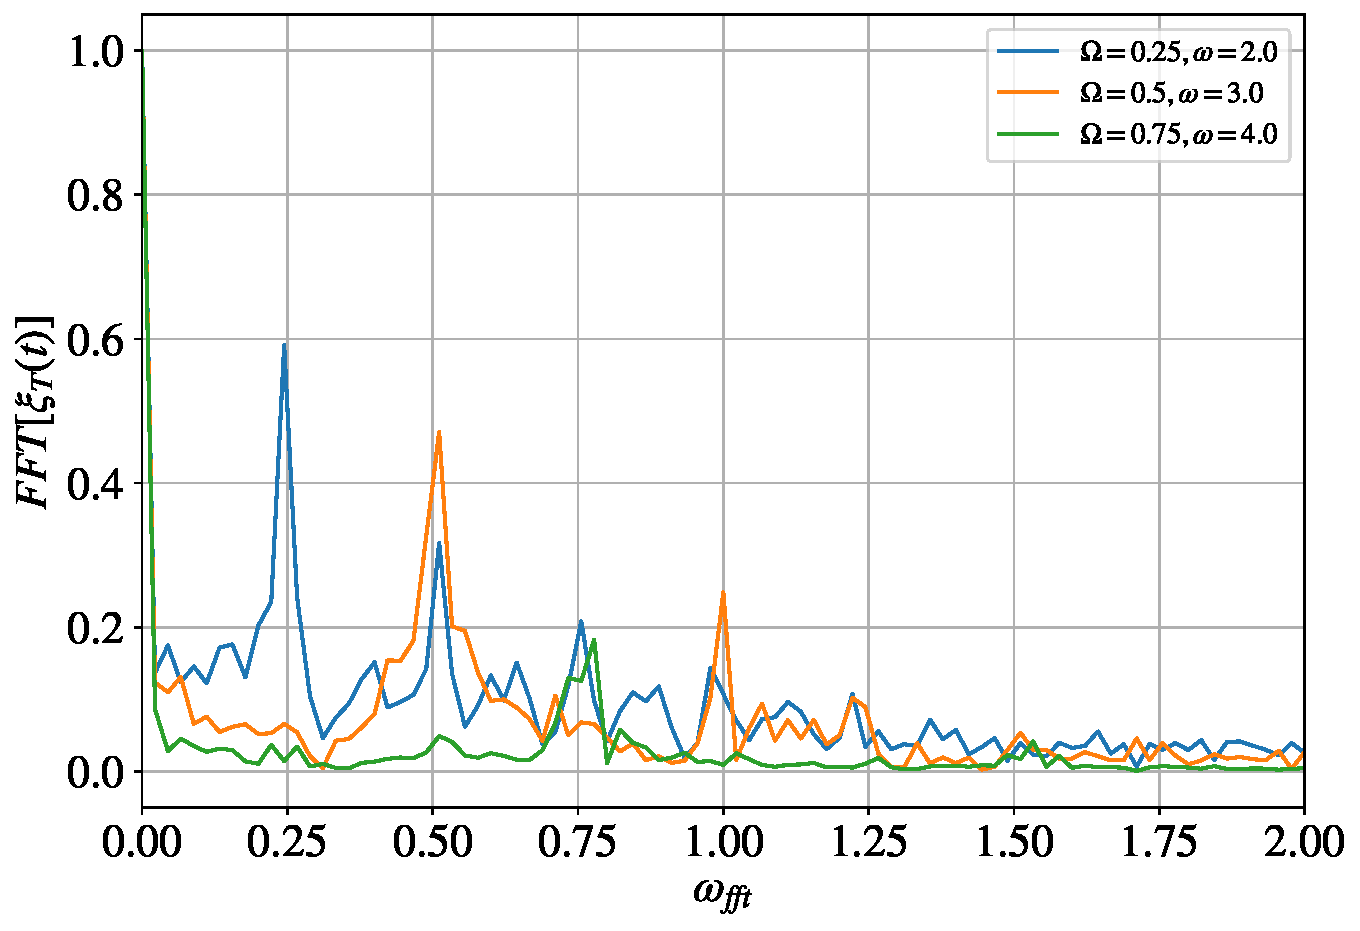
\includegraphics[scale=0.38]{images/spectra_xi_diff_omegas.pdf}
    \caption{Normalized Fourier spectra of the signal $\xi_T(t)$ with $t \in (T,T_f)$ for three different combinations of $\Omega$ and $\omega$, using $\delta t = 10^{-4}$. In each time-evolution the laser source was left active for $t \in (0, T)$ and then switched off for $t\in(T,T_f)$, being $T=10\pi$ and $T_f=100\pi$. The coefficient matrix used as initial condition for the time evolution corresponds to the resulting one from the convergence of the time-independent solver with $\delta=10^{-6}$.}
    \label{fig:fourier_spectra_xi}
\end{figure}
}

\begin{figure*}[h!]
    \centering
    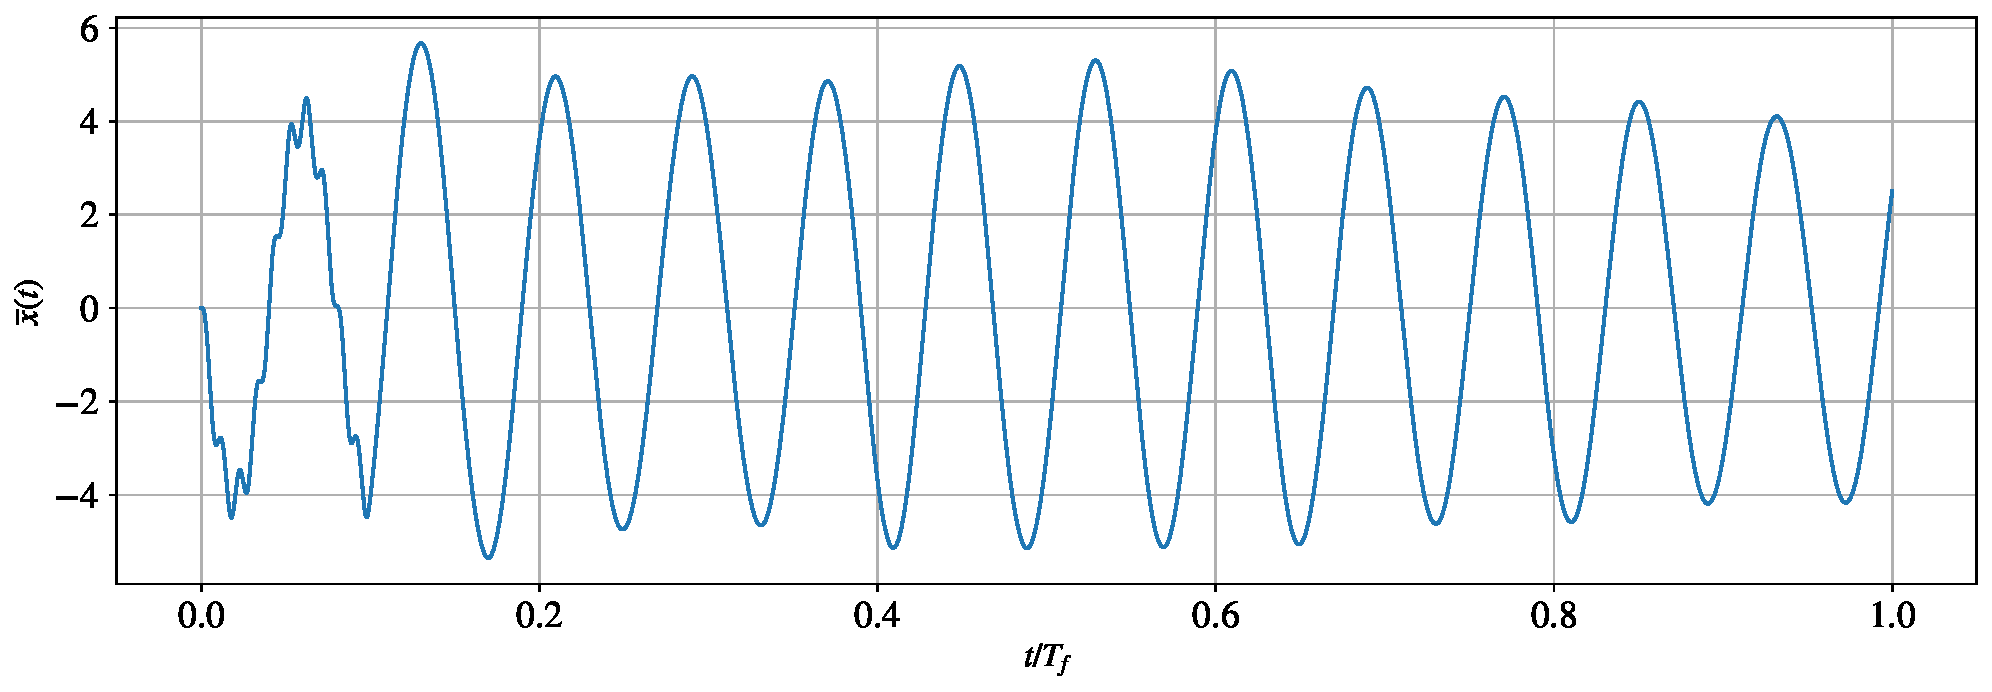
\includegraphics[scale=0.5]{images/dipole_laser_ONOFF.pdf}
    \caption{Time evolution of $\overline{x}(t)$ (see Eq.\,\ref{eq:x_time_dependent_coeff}) with laser source active for $t\in(0, 10 \pi)$ and then switched off up to $T_f=100\pi$. The coefficient matrix used as initial condition for the time evolution corresponds to the resulting one from the convergence of the time-independent solver with $\delta=10^{-6}$. Plotted results are referred to a system with $\Omega=0.25$ and $\omega=2$ and the time step used is $\delta t = 10^{-4}$. }
    \label{fig:laser_on_off}
\end{figure*}

\begin{figure*}[h!]
    \centering
    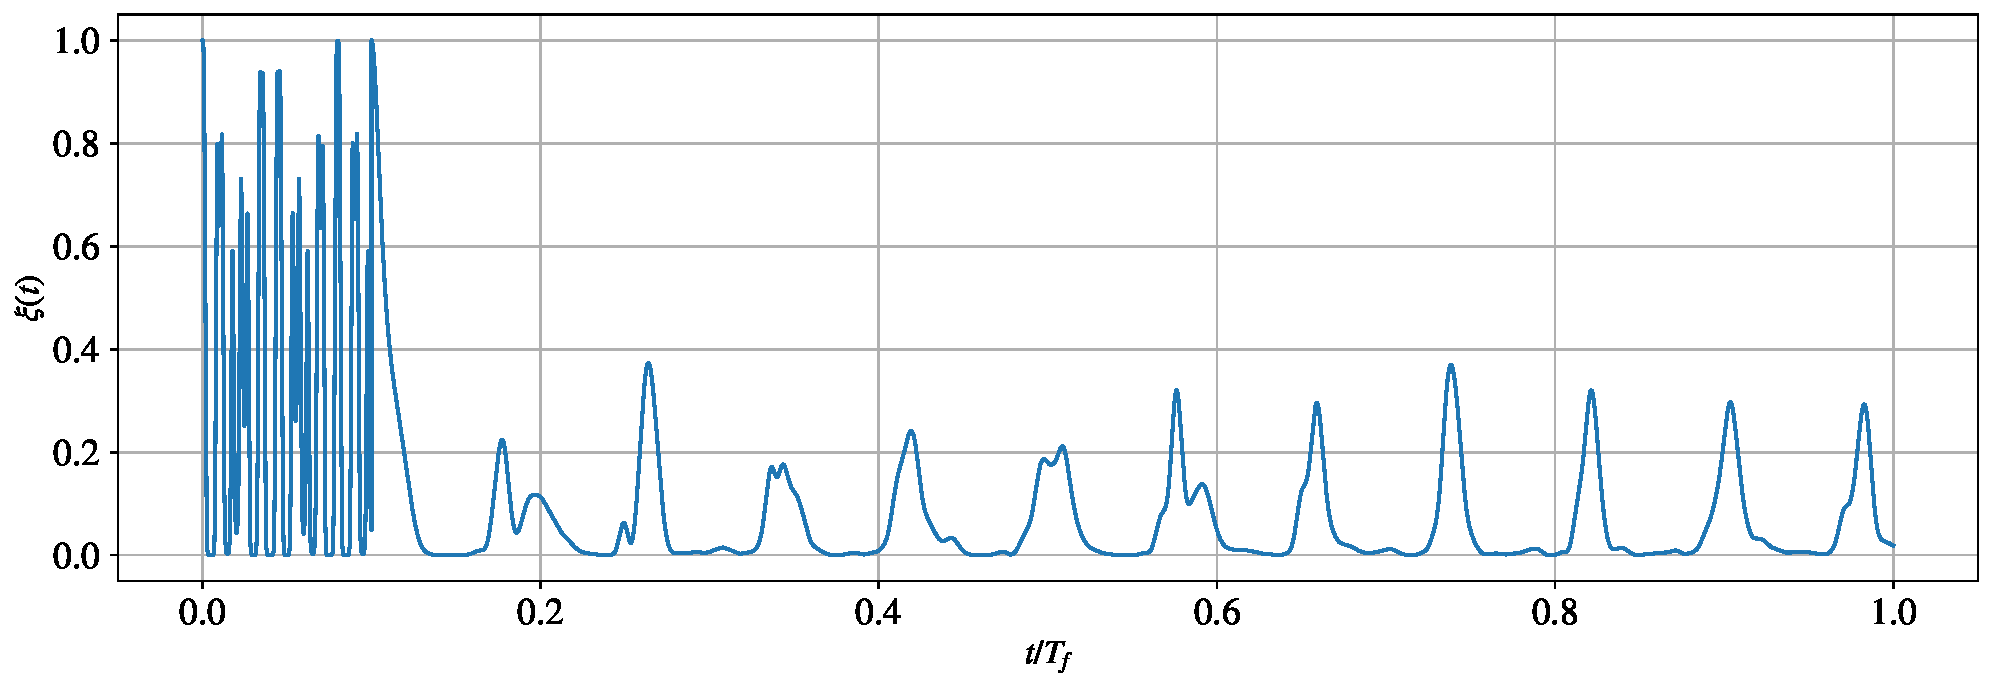
\includegraphics[scale=0.5]{images/overlap_laser_ONOFF.pdf}
    \caption{Time evolution of $\xi (t)=\vert \braket{\Psi(t)}{\Psi(0)} \vert^2$ for $t/T_f<0.1$ and $\xi_T (t)=\vert \braket{\Psi(t)}{\Psi(T)} \vert^2$ for $t/T_f>0.1$ with laser source active for $t\in(0, 10 \pi)$ and then switched off up to $T_f=100\pi$. The coefficient matrix used as initial condition for the time evolution corresponds to the resulting one from the convergence of the time-independent solver with $\delta=10^{-6}$. Plotted results are referred to a system with $\Omega=0.25$ and $\omega=2$  and the time step used is $\delta t = 10^{-4}$. }
    \label{fig:overlap_T}
\end{figure*}

